
\clearpage 
\section{ 算法 }

\subsection{ Edge Function }
Juan Pineda \cite{EdgeFunction} 在他论文提出的概念,就是\textbf{barycentric coordinates}的应用。
它在计算三角形属性方面上有很大的优势,如深度z-depth、颜色color、纹理坐标uv、法线等插值计算。
重心(质心)坐标的应用主要体现在:
\begin {itemize}
    \item {判断一个点是否在三角形内}
    \item {根据三角形三个顶点得到三角形内一个点P}
\end {itemize}
在软光栅化或光线追踪都用得到。

\begin{figure}[h]
    \centering
    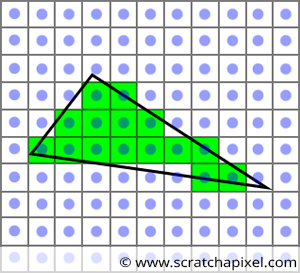
\includegraphics[width=0.25\textwidth]{images/rasterization-triangle1}
    \hspace{0.1cm}
    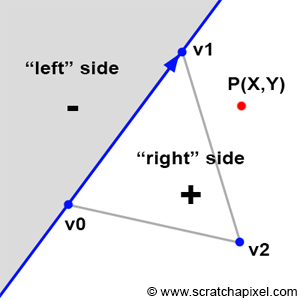
\includegraphics[width=0.25\textwidth]{images/rasterization-triangle2}
    \hspace{0.1cm}
    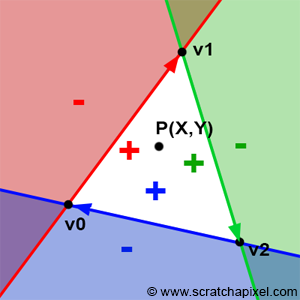
\includegraphics[width=0.25\textwidth]{images/rasterization-triangle3}
    \caption{左边:测试像素是否覆盖三角形,是光栅化算法的原理;
    中间:判断点与线的关系,大于0在右边,小于0在左边,等于0在线上;
    右边:在白色区域中的点都是位于三角形边的右边
    }    
\end{figure}
遍历整个FrameBuffer去判断点是不是在在三角形内部,太浪费时间去遍历不可能的结果了。
\begin{figure}[h]
    \centering
    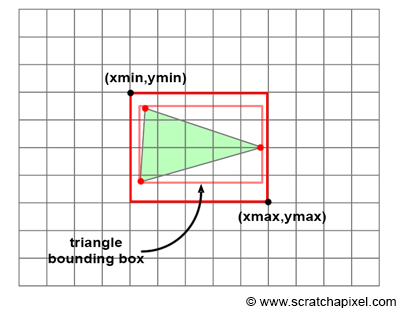
\includegraphics[width=0.3\textwidth]{images/rasterization-boundingbox.png}
    \caption {三角形的顶点告诉了大致范围,减少遍历的次数,提高访问性能}
\end{figure}
计算boundingbox的算法很简单,速度也快。

\subsection{Reconstructing Position From Depth}
需求:根据当前像素的Depth计算出View空间中的Position
先分析depth是如何计算出来的,在vertex shadeer中
\begin{lstlisting}
    outPos = mul(inPos, mvp);
    outDepth.xy = outPos.zw;
\end{lstlisting}
在pixel shader中,
\begin{lstlisting}
    depth = outDepth.x / outDepth.y;
\end{lstlisting}
按照这个过程逆运算回去
\begin{lstlisting}
    z = texture(depthSampler, inUV);
    x = inUV.x * 2 - 1;
    y = (1 - inUV.y) * 2 - 1;
    pos = (x,y,z,1)
    pos = mul(pos, mvpInverse);
    pos = pos.xyz / pos.w;
\end{lstlisting}
但是存在一些问题
\begin{itemize}
    \item {z/w是非线性分布的,经过RTT(Render To Texture)后再变换回去,精度存在误差}
    \item {计算量大}
\end{itemize}
从物理状态来看看摄像机的视锥体的抽象形式,从摄像机位置到远裁剪面发射一条射线,存在一个关系:

\begin{figure}[h]
    \centering
    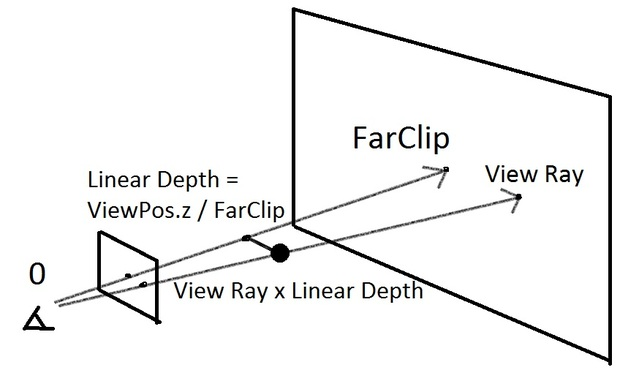
\includegraphics[width=0.5\textwidth]{images/reconstructing-position-from-depth.png}
\end{figure}

\begin{lstlisting}
    posView = viewRayDir * linearDepth;    
    linearDepth = posView.z / farClipDistance;
\end{lstlisting}

linearDepth是规格化的Z值,它满足线性分布。现在的问题就如何得到RayDir向量了。在View空间中,摄像机的位置是(0,0,0),
对于可见的每个点,从摄像机出发的射线都与远裁剪面相交,交点就是方向向量RayDir的坐标。由图中可知,是利用中心线和射线组成的三角形,满足等比关系,是线性关系。
远裁剪面的四个顶点是可以计算出来的,思路就出来了。

\begin{itemize}
    \item {1. 把posView.z/farClipDistance的值保存到RTT中,得到的值满足线性关系}
    \item {2. 从RTT中得到linearDepth, 从vertex shader中得到viewRayDire.xy, }
\end{itemize}

\begin{lstlisting}
    viewRayDir = float3(farClip.x, farClip.y, farClipDistance);
    posView = viewRayDir * linearDepth;
\end{lstlisting}

\subsection{Trackball}
轨迹球\cite{Trackball}
轨迹球就是在屏幕之外虚构一个球形曲面,使鼠标在二维屏幕上的移动投影到球形曲面上。
即一个半球覆盖在屏幕上面。以屏幕中心为球心O,X轴向右,Y轴向上,Z轴向外。当鼠标在球面的范围内移动时,可以由二维屏幕上的二维左边点P(x,y),通过数学关系求得其在球面上的投影点P'。
鼠标从P1移动到P2,对应的球面就是从P1'到P2'。产生两个向量V1=OP1',V2=OP2',  
V1与V2的叉乘得到向量N,即三维物体的旋转轴,V1到V2的转角量就是三维物体的旋转角度。
屏幕时矩形,球形的投影在屏幕的平面上只会是一个圆,总会有些区域的点投影后会落在球面之外。
